
\documentclass[draft,linenumbers]{agujournal2019}

\usepackage{url} 
\usepackage{lineno}
\usepackage[inline]{trackchanges} 
\usepackage{soul}
\usepackage{natbib}
\usepackage{float}

%\draftfalse

\journalname{JGR Oceans}

%% Possible journal
%%% JGR oceans?

%%%%%%%%%%%%%%%%%%%%%%%%%%%%%%%%%%%

%% MACROS
\newcommand{\MKE}{\overline{\textrm{KE}}}
\newcommand{\KE}{\textrm{KE}}
\newcommand{\MEKE}{\overline{\textrm{EKE}}}
\newcommand{\EKE}{\textrm{EKE}}
\newcommand{\MCEKE}{\overline{\textrm{CEKE}}}
\newcommand{\CEKE}{\textrm{CEKE}}
\newcommand{\MnCEKE}{\overline{\textrm{nCEKE}}}
\newcommand{\nCEKE}{\textrm{nCEKE}}
\newcommand{\cEddy}{\textrm{cEddy}}

\begin{document}
\title{Climatology, seasonality and trends of oceanic coherent eddies}

\authors{Josu\'e Mart\'inez-Moreno\affil{1}, Andrew McC. Hogg\affil{1}, and Matthew England\affil{2}}
\affiliation{1}{Research School of Earth Science and ARC Center of Excellence for Climate Extremes, Australian National University, Canberra, Australia}
\affiliation{2}{Climate Change Research Centre (CCRC), UNSW Australia, Sydney NSW, Australia}

\correspondingauthor{Josu\'e Mart\'inez-Moreno}{josue.martinezmoreno@anu.edu.au}

\begin{keypoints}
	% \item Kinetic energy climatology reveals a surprising heterogeneity in the global ocean.
	% \item Transient kinetic energy show significant increasing trends over large areas of the Southern Ocean and the Northern Hemisphere.
	% \item Regional kinetic energy climatology strongly depends to the region dominant oceanic process.
	\item Kinetic energy of coherent eddies contain around 30\% of the surface ocean kinetic energy budget.
	\item Seasonal cycle of the number of coherent eddies and coherent eddy amplitude reveal a 3-6 month lag to wind forcing
	\item The coherent eddy amplitude has increase at a rate of 3 cm per decade since 1993.
\end{keypoints}


\begin{abstract}
	
	Ocean eddies influence regional and global climate through mixing and transport of heat and properties. One of the most recognizable and ubiquitous feature of oceanic eddies are vortices with spatial scales of tens to hundreds of kilometers, frequently referred as ``mesoscale eddies" or ``coherent eddies". Coherent eddies are known to transport properties across the ocean and to locally affect near-surface wind, cloud properties and rainfall patterns. Although coherent eddies are ubiquitous, yet their climatology, seasonality and long-term temporal evolution remains poorly understood. Thus, we examine the kinetic energy contained by coherent eddies and we present the annual, interannual, and long-term changes of automatically identified coherent eddies from satellite observations and a state of the art numerical simulation from 1993 to 2018. Satellite observations show that around 40\% of the kinetic energy contained by ocean eddies corresponds to coherent eddies. Additionally, a strong hemispherical seasonal cycle is observed, on top of a 3--6 months lag between the wind forcing and the response of the coherent eddy field. Furthermore, the seasonality of the number of coherent eddies and their amplitude reveals that the number of coherent eddies responds faster to the forcing ($\sim$3 months), while the coherent eddy amplitude is lagged by $\sim$6 months.  There are regions that show a pronounced influence of coherent eddies, notably, the East Indian Ocean, the East Tropical Pacific Ocean, and the South Atlantic Ocean. In these locations, a strong seasonal cycle and interannual variability can be observed in both satellite and numerical models. Although, there is agreement between these products on the seasonality of the number of eddies, the seasonality of the coherent eddy amplitude between these products show some inconsistencies. Long-term trends of the coherent eddy amplitude from satellite observations and the state of the art model show significant increases in the eddy amplitude of $\sim$3cm per decade in large portions of the ocean, while the number of coherent eddies remains constant. Our analysis highlight the relative importance of the coherent eddy fiend in the ocean kinetic energy budget, imply a strong response of the eddy number and eddy amplitude to the surface wind at different time-scales, and showcases for the first time seasonality, and multidecadal trends of the coherent eddy properties. 

	\noindent\textbf{Plain summary}
	
\end{abstract}	

% -	Ratios of KE!! 
% -	Coherent signature + seasonality  and non-coherent signature (not key point)
% -	Identify regions dominated by coherent eddies
	
\section{Introduction}

Mesoscale ocean variability with spatial scales of tens to hundreds of kilometers is the most energetic scale in the ocean and comprises processes such as vortices, waves, and jets. In particularly, one of the most recognizable mesoscale process are vortices. Although, in literature mesoscale vortices are commonly refer as "mesoscale eddies", this term is often used to describe mesoscale ocean variability, thus, where we will use the term coherent eddy to refer to coherent vortices. 

Coherent eddies bla bla bla






% Ocean eddies explain most of the temporal variability 


% of kinetic energy ($\KE$) and transport of tracers in the oceans. KE associated with mesoscale variability is commonly used as a diagnostic of the ocean state from satellite observations and numerical simulations.


% Ocean currents 

%Ocean currents are highly anisotropic and include coherent vortices and meandering jets. While coherent vortices (recirculating currents) are approximated as ellipses with axes smaller than the Rossby radius of deformation ($R_D$), meandering jets are narrow but elongated currents. The anisotropic nature of these features translates in ...


% %	Oceans are fundamental in the regulation of the climate system, as they have the capacity to absorb and transport heat, carbon, and other tracers through diverse flow scales which range from planetary (thermohaline circulation) to microscopic scales (turbulence). Mesoscale processes (hundreds of kilometres in scale) explain most of the temporal variability of kinetic energy (KE) and transport of tracers in the oceans. KE associated with mesoscale variability is commonly used as a diagnostic of the ocean state from satellite observations and numerical simulations.  
% %	
% %	Mean KE indicates regions in the ocean with persistent large scale circulation \citep{}, while the temporal variability of the KE field are directly linked to many transitory process in the ocean: coherent vortices, meanders, and waves. Transient events are strongly dependent to surface forcing and mixed layer variability \citep{}. 
% %	
% %	The transient component of the variability includes seasonal, inter-annual, and decadal variability \citep{}. 
% %	
% %	It has been reported an significant increase of the eddy kinetic energy (EKE) in the Southern Ocean \citep{}, 
% %	
% %	
% %	Add something here
% %	however the spatial variability is still unknown. 
% %	
% %	Despite satellite observations being coarser than 0.25$^\circ$ in many areas of the ocean, and a lack of studies exploring the global KE climatology, the present study will expands the understanding on surface ocean variability, and it is crucial  for ocean modeling community not only for ocean model validation, but also to  improve the eddy parametrization. 
% %	
% %	This study differs to \citet{Kang_On_2017} as we compute global climatologic focusing in the spatial distribution instead of the purely seasonality cycle.  The main goal of the present work is to generate a global climatology from the latest satellite observation dataset available, in order to complement the known information of the variability of the superficial Kinetic Energy.
% %	
% %	The data sources and methodology are described in section \ref{sec:Methods}. Global seasonality, inter-annual variability and trends are explored in sections \ref{sec:R_season},  \ref{sec:R_variability}, and  \ref{sec:R_trends} respectively. In section \ref{sec:R_regional} we present 3 regions in which we further investigate the temporal variability of kinetic energy and each of its components.
% %	
	\section{Methods}
	\label{sec:Methods}
% %	
% %	We compute global climatological montly KE, EKE, TEKE and TRKE by processing satellite observations and implementing TrackEddy an coherent eddy identification-reconstruction algorithm, with the capability to separate the Kinetic Energy from coherent and non-coherent features. The present study expands our understanding in the seasonal cycle, inter-annual variability and decadal trends.
% %	
% %	
	\subsection{Kinetic Energy decomposition}

	Kinetic energy is commonly divided into the mean and temporal variability components through a Reynolds decomposition. At a given time, the velocity field ($\mathbf{u}$) is split into the time mean ($\mathbf{\overline{u}}$) and time varying components ($\mathbf{u'}$). Additionally, as part of the climatology we also further decompose the eddy kinetic energy into the eddy kinetic energy contained by coherent features ($\mathbf{u'_e}$) and non-coherent ($\mathbf{u'_n}$). Therefore the KE equation can be written as:
	
	\begin{equation}
		\mathrm{KE}= \mathbf{\overline{u}}^2 +\underbrace{ \mathbf{u'_e}^2+ \mathbf{u'_n}^2 + \mathcal{O}^2}_{\mathbf{u'}^2}
	\end{equation}
	
	The second order terms ($\mathcal{O}$) are negligible as their time average is two orders of magnitude smaller than any other term. For more information about the decomposition of the field into coherent features and non-coherent features refer to \citet{Martinez_Kinetic_2019}.
% %	
% %	Qualitatively KE seasonality is similar to TKE and therefore we will focus mostly on the seasonality of TKE.

	\section{Results}
	\label{sec:Results}
	
	\subsection{Coherent Eddy Energetics}
	\label{subsec:R_season}
	
	\subsubsection{Global}

	\begin{figure}
	    \centering
	    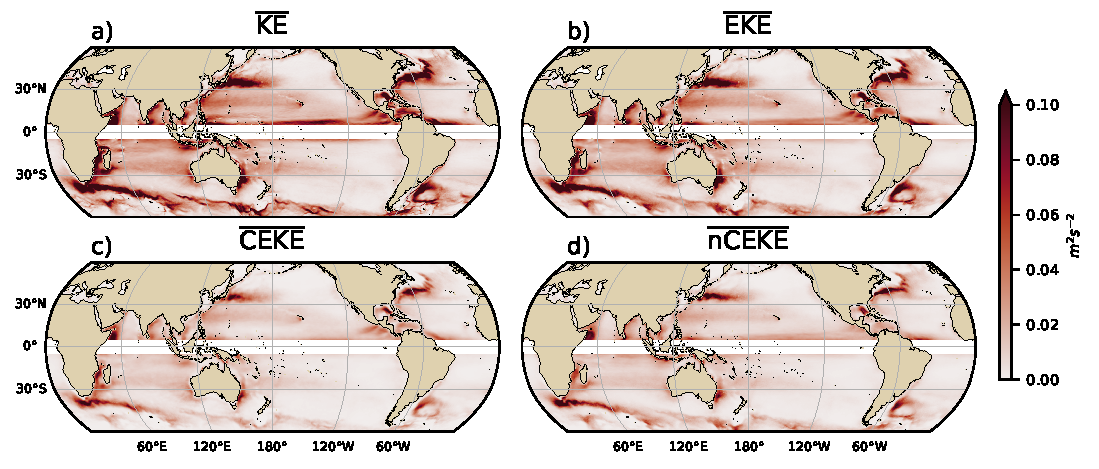
\includegraphics[width=1\textwidth]{figures/mean_ke_maps_satellite.pdf}
	    \caption{Climatology of surface kinetic energy ($\MKE$), surface eddy kinetic energy ($\MEKE$), surface coherent eddy kinetic energy ($\MCEKE$), and surface non-coherent eddy kinetic energy ($\MnCEKE$) between 1993-2018.}
	    \label{fig:eddy_climatology}
	\end{figure}
	
	% mean surface eddy kinetic energy (EKE)
	% 364 and surface eddy kinetic energy trend between 1993-2020 (a) Zonally averaged SSH
	% 365 trend; (b) map of SSH trend (92.1% of area is statistically significant above the 95% con-
	% 366 fidence level; for spatial distribution refer to Extended Data Fig. 1a); (c) zonally averaged
	% 367 mean EKE; (d) map of mean EKE; (e) zonally averaged EKE trend; (f) map of EKE trend
	% 368 (55.4% of area is statistically significant above the 95% confidence level; see Extended
	% 369 Data Fig. 1b).

	\begin{itemize}
		\item Figure 1 shows regions with high values of Kinetic Energy at the Western Boundary Currents, ACC, and ocean gyres. 
		\item $\MEKE$ Explains $~70\%$ of $\MKE$, while $\MCEKE$ is $~40\%$ of $\MEKE$ and $\MnCEKE$  is $~60\%$ of $\MEKE$ 
		\item Maps show that $\MKE$, $\MEKE$, $\MCEKE$, and $\MnCEKE$ are dominated by the western boundary currents, the Antarctic Circumpolar Current (ACC).
	\end{itemize}
	
	\begin{figure}
	    \centering
	    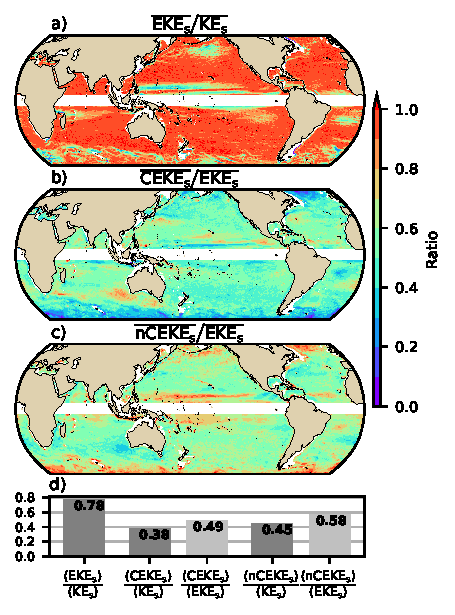
\includegraphics[width=1\textwidth]{figures/eke_ratio_map_all.pdf}
	    \caption{Ratios of the kinetic energy components. a) Map of the proportion of mean eddy kinetic energy ($\EKE$) versus mean kinetic energy ($\MKE$);
		b) Map of the proportion of mean coherent eddy kinetic energy ($\MCEKE$) versus mean eddy kinetic energy ($\MEKE$);
		c) Map of the proportion of mean non-coherent eddy kinetic energy ($\MnCEKE$) versus mean eddy kinetic energy ($\MEKE$);
		d) Global ratios of mean eddy kinetic energy ($\left<\MEKE\right>$), mean coherent eddy kinetic energy ($\left<\MCEKE\right>$) and mean non coherent eddy kinetic energy ($\left<\MnCEKE\right>$) versus the global mean kinetic energy ($\left<\MKE\right>$) and global mean eddy kinetic energy ($\left<\MEKE\right>$).
		}
	    \label{fig:eddy_ratio}
	\end{figure}

	Note that \nCEKE has a large amount of energy at high latitudes, this could be a consequence of the satellites not resolving the mesoscale coherent eddies. 

	\subsubsection{Seasonality}

	\begin{figure}
	    \centering
	    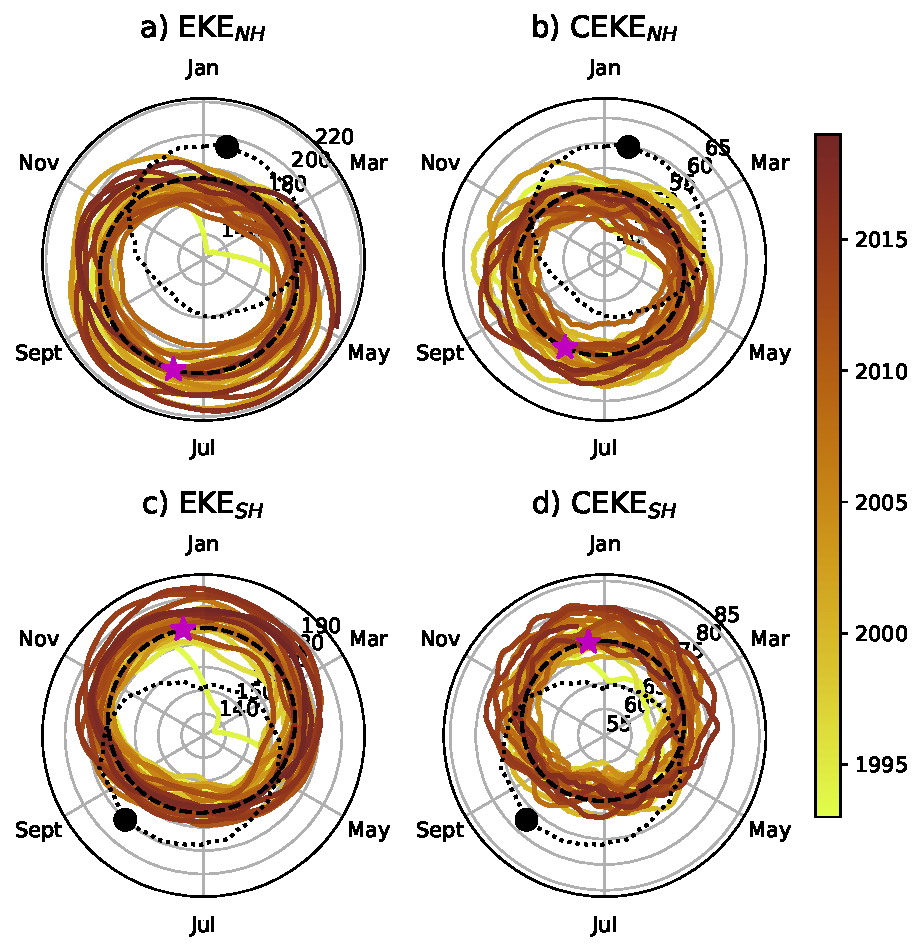
\includegraphics[width=1\textwidth]{figures/All_polar_plots.pdf}
	    \caption{Hemispherical seasonality of eddy kinetic energy ($\EKE$), coherent eddy kinetic energy ($\CEKE$), and non-coherent eddy kinetic energy ($\CEKE$). Panels a,b and c show the northern hemisphere seasonal cycle, while panels d,e, and f correspond to the southern hemisphere. Dashed lines correspond to the seasonal climatology of the fields and dotted lines show the climatology of the wind magnitude. The green and magenta stars show the maximum of the seasonal cycle for the kinetic energy components and the wind magnitude, respectively. The line colors show the year.}
	    \label{fig:eddy_energy_polar}
	\end{figure}
	
	\subsection{Coherent Eddy Statistics}

	\subsubsection{Global}
	
	\textbf{Make sure to mention dipoles in the boundary currents.}

    \begin{itemize}
		\item 
	\end{itemize}

	\begin{figure}
	    \centering
	    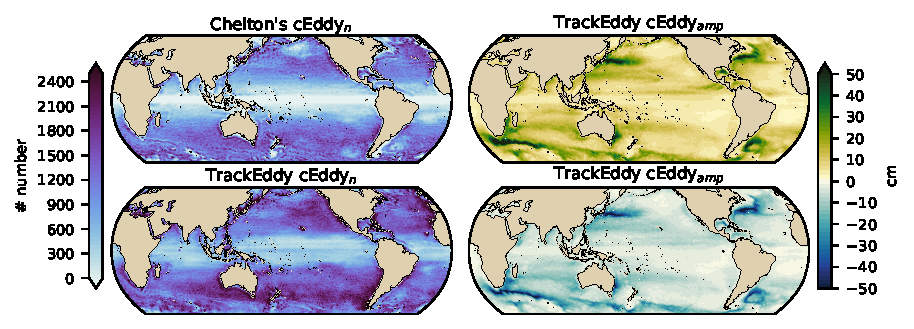
\includegraphics[width=1\textwidth]{figures/global_stats_polarity.pdf}
	    \caption{Climatology of the coherent eddy statistics. a) Climatology of the number of coherent eddies ($\cEddy_n$) identified by \citet{Chelton_Global_2007}; b) Climatology of the warm core coherent eddy amplitude ($\cEddy_{amp}$). c) Climatology of the number of coherent eddies ($\cEddy_n$) identified by \citet{Martinez_Kinetic_2019}; d) Climatology of the cold core coherent eddy amplitude ($\cEddy_amp$).}
	    \label{fig:eddy_stats_climatology}
	\end{figure}

	Although these algorithms use different identification criteria, the spatial pattern of the number of eddies in consistent between them.

	The maximum positive coherent eddy amplitude is commonly located polewards of the mayor boundary currents, while the maximum negative coherent eddy amplitude is found equatorwards. This is consistent to how coherent eddies are shed from these boundary currents.

	\subsubsection{Seasonality}

	\begin{figure}
	    \centering
	    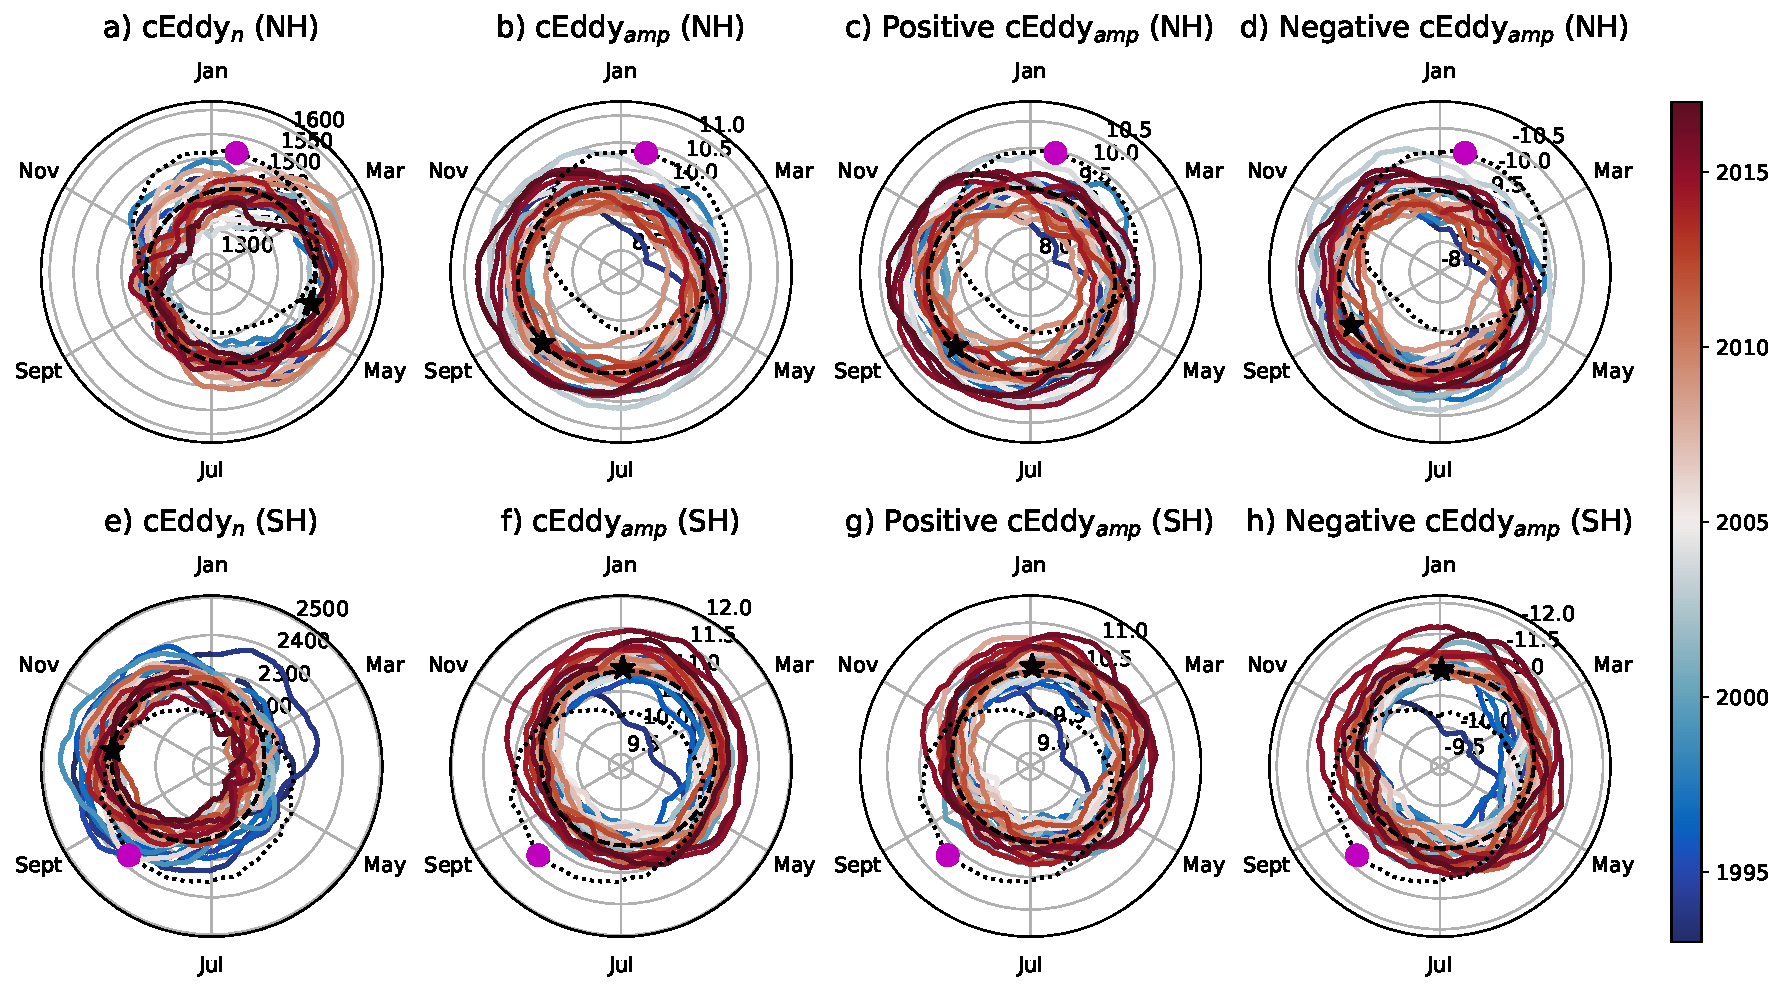
\includegraphics[width=1\textwidth]{figures/All_polar_plots_eddy_stats_polarity.pdf}
	    \caption{Hemispherical seasonality of the coherent eddy statistics;
		a,e) seasonal cycle of the number of coherent eddies ($\cEddy_n$); b,f) seasonal cycle of the mean coherent eddy amplitude ($\cEddy_{amp}$); c,g) seasonal cycle of the warm core coherent eddies amplitude (\textbf{w$\cEddy_{amp}$}); d,h) seasonal cycle of the cold core coherent eddies amplitude (\textbf{c$\cEddy_{amp}$}). Panels a,b and c show the northern hemisphere seasonal cycle, while panels d,e, and f correspond to the southern hemisphere. Dashed lines correspond to the seasonal climatology of the fields and dotted lines show the climatology of the wind magnitude. The green and magenta stars show the maximum of the seasonal cycle for the kinetic energy components and the wind magnitude, respectively. The line colors show the year.}
	    \label{fig:eddy_stats_polar}
	\end{figure}


	\subsection{Regional}
	
	\begin{figure}
	    \centering
	    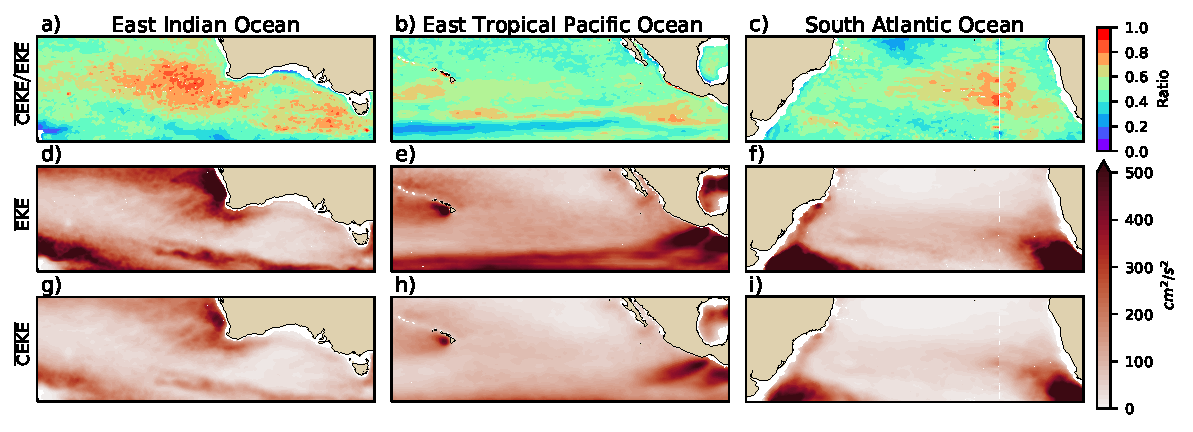
\includegraphics[width=1\textwidth]{figures/regional_eke_ceke_stats_no_stats.pdf}
	    \caption{Climatology of regional statistics of the eddy field and coherent eddy field for the East Indian Ocean, East Tropical Pacific Ocean and South Atlantic Ocean. a-c) Ratio of coherent eddy kinetic energy $\CEKE$ versus eddy kinetic energy $\EKE$; d-f)  mean eddy kinetic energy ($\MEKE$); g-i) mean coherent eddy kinetic energy ($\MCEKE$).}
	    \label{fig:regional_energy_ratios}
	\end{figure}


	\begin{figure}
	    \centering
	    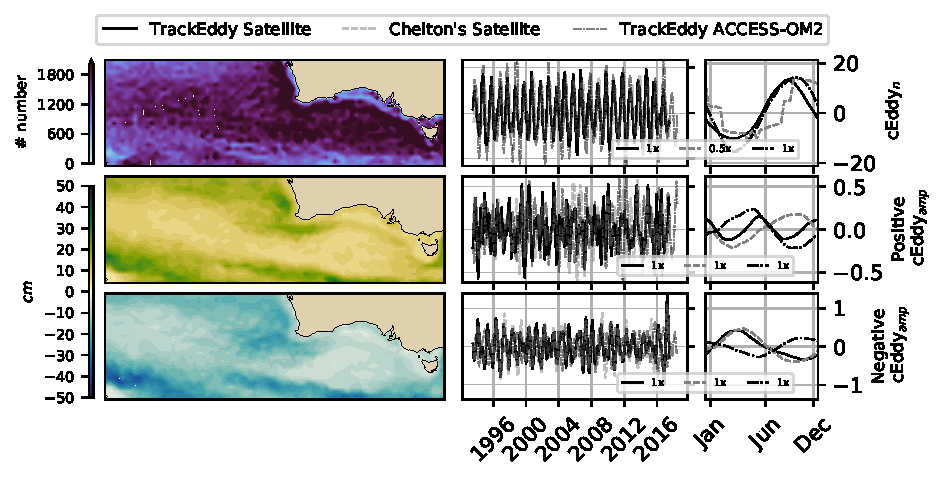
\includegraphics[width=1\textwidth]{figures/regional_eke_ceke_stats_0.pdf}
	    \caption{Climatology of regional statistics of the eddy field and coherent eddy field for the East Indian Ocean, East Tropical Pacific Ocean and South Atlantic Ocean. a-c Zoom to ratio of CEKE and EKE; d-f  mean eddy kinetic energy ($\MEKE$); g-i mean coherent eddy kinetic energy ($\MCEKE$); j-k count of identified coherent eddies between 1993-2019; and l-n mean coherent eddy amplitude between 1993-2019.}
	    \label{fig:east_indian_cycle}
	\end{figure}

	Number 295.85546403962104
	Pos amp 0.12094501820533601
	Neg amp -0.1385068018754378
	Chelton Number 236.7010877964295
	Chelton Pos amp 7.779538694987785
	Chelton Neg amp -10.075637745571715
	ACCESS Number 315.24697840283096
	ACCESS Pos amp 0.0875635001289238
	ACCESS Neg amp -0.08147261526708122

	\begin{figure}
	    \centering
	    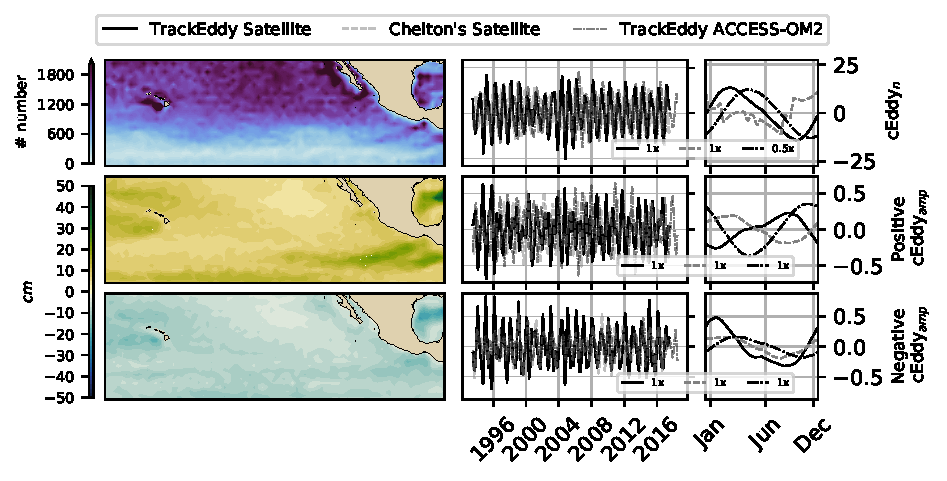
\includegraphics[width=1\textwidth]{figures/regional_eke_ceke_stats_1.pdf}
	    \caption{Climatology of regional statistics of the eddy field and coherent eddy field for the East Indian Ocean, East Tropical Pacific Ocean and South Atlantic Ocean. a-c Zoom to ratio of CEKE and EKE; d-f  mean eddy kinetic energy ($\MEKE$); g-i mean coherent eddy kinetic energy ($\MCEKE$); j-k count of identified coherent eddies between 1993-2019; and l-n mean coherent eddy amplitude between 1993-2019.}
	    \label{fig:east_tropical_cycle}
	\end{figure}

	Number 207.37973697877084
	Pos amp 0.08901200544912018
	Neg amp -0.08816744392087235
	Chelton Number 155.8983449906741
	Chelton Pos amp 5.461227370020861
	Chelton Neg amp -5.348246201100335
	ACCESS Number 243.4991508883295
	ACCESS Pos amp 0.05249108358772637
	ACCESS Neg amp -0.04136883487182314

	\begin{figure}
	    \centering
	    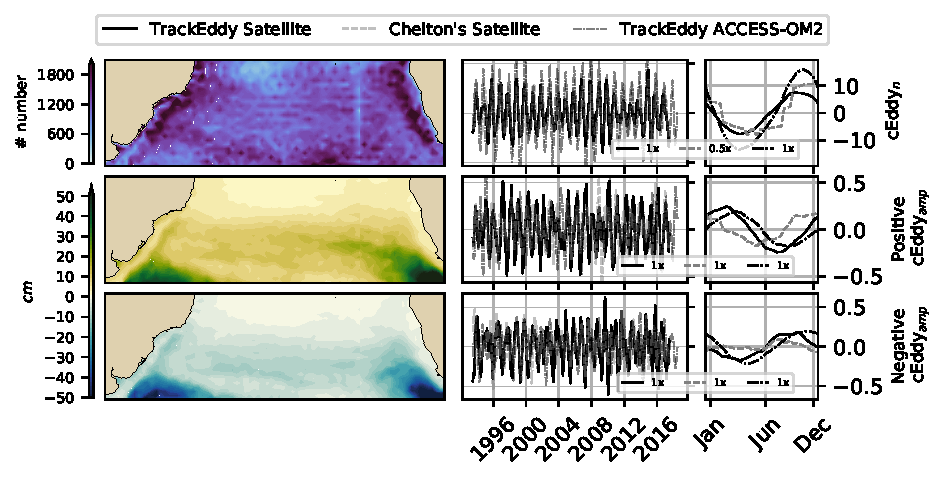
\includegraphics[width=1\textwidth]{figures/regional_eke_ceke_stats_2.pdf}
	    \caption{Climatology of regional statistics of the eddy field and coherent eddy field for the East Indian Ocean, East Tropical Pacific Ocean and South Atlantic Ocean. a-c Zoom to ratio of CEKE and EKE; d-f  mean eddy kinetic energy ($\MEKE$); g-i mean coherent eddy kinetic energy ($\MCEKE$); j-k count of identified coherent eddies between 1993-2019; and l-n mean coherent eddy amplitude between 1993-2019.}
	    \label{fig:south_atlantic_cycle}
	\end{figure}

	Number 228.35682569539446
	Pos amp 0.084251050110757
	Neg amp -0.08530413757977995
	Chelton Number 170.22168598454567
	Chelton Pos amp 5.291564971943509
	Chelton Neg amp -5.128095846325381
	ACCESS Number 311.68099516009386
	ACCESS Pos amp 0.06803317095123791
	ACCESS Neg amp -0.04969146684717923


	Overall, we observe a polewards decrease in the number of the eddies. This supports the idea that the satellite observations are consistent with a continue dataset.

	% Global 
	% - Climatology
	% - Seasonality 

	% Regions
	% 	Individual regions

	% Show positive vs negative amplitudes

	\section{Trends}

	\begin{figure}
	    \centering
	    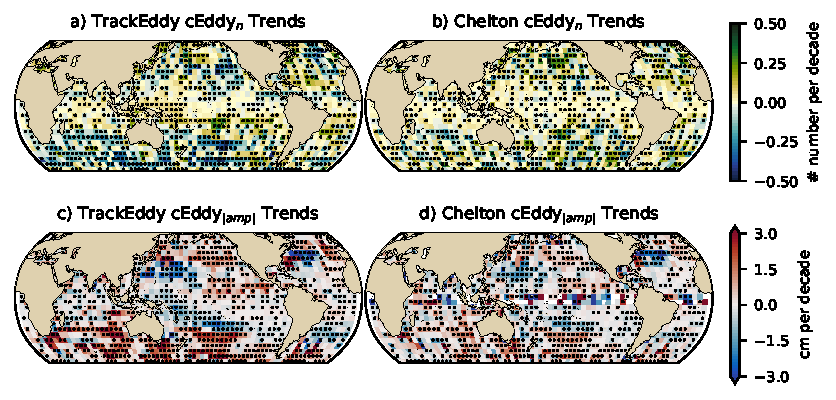
\includegraphics[width=1\textwidth]{figures/all_trackeddy_trends.pdf}
	    \caption{Trends of coherent eddy statistics. a,b and c Trends of the number of identified coherent eddies from satellite observations identified using TrackEddy, satellite observations identified using Chelton's, and state of the art numerical simulation identified using TrackEddy. d,e and f Trends of the sum of the absolute value of identified coherent eddies amplitude from satellite observations identified using TrackEddy, satellite observations identified using Chelton's, and state of the art numerical simulation identified using TrackEddy. Gray stippling shows regions that are statistically significant above the 95\% confidence level.
		}
	    \label{fig:eddy_stats_trends}
	\end{figure}
	
	\section{Summary and Conclusions}	
	
	\acknowledgments
	
	\bibliography{biblio.bib}
	
\end{document}
